\let\negmedspace\undefined
\let\negthickspace\undefined
\documentclass[journal]{IEEEtran}
\usepackage[a5paper, margin=10mm, onecolumn]{geometry}
\usepackage{tfrupee} 

\setlength{\headheight}{1cm} 
\setlength{\headsep}{0mm}  
\usepackage{gvv-book}
\usepackage{gvv}
\usepackage{cite}
\usepackage{amsmath,amssymb,amsfonts,amsthm}
\usepackage{algorithmic}
\usepackage{graphicx}
\usepackage{textcomp}
\usepackage{xcolor}
\usepackage{txfonts}
\usepackage{listings}
\usepackage{enumitem}
\usepackage{mathtools}
\usepackage{gensymb}
\usepackage{comment}
\usepackage[breaklinks=true]{hyperref}
\usepackage{tkz-euclide} 
\usepackage{listings}
% \usepackage{gvv}                                        
\def\inputGnumericTable{}                                 
\usepackage[latin1]{inputenc}                                
\usepackage{color}                                            
\usepackage{array}                                            
\usepackage{longtable}                                       
\usepackage{calc}                                             
\usepackage{multirow}                                         
\usepackage{hhline}                                           
\usepackage{ifthen}                                           
\usepackage{lscape}
\usepackage{tikz}
\usetikzlibrary{patterns}
\begin{document}

\bibliographystyle{IEEEtran}
\vspace{3cm}


\title{GATE 2016 MN }
\author{ai25btech11039
- Harichandana Varanasi}
\maketitle
% \maketitle
% \newpage
% \bigskip
{\let\newpage\relax\maketitle}

\renewcommand{\thefigure}{\theenumi}
\renewcommand{\thetable}{\theenumi}
\setlength{\intextsep}{10pt} % Space between text and floats
\noindent\textbf{Q.1 -- Q.5 carry one mark each.}
\vspace{0.5em}
\begin{enumerate}[leftmargin=0pt]
% Q1
\item The volume of a sphere of diameter $1$ unit is \underline{\hspace{1.5cm}} than the volume of a cube of side $1$ unit.
  \begin{enumerate}
    \begin{multicols}{4}
        \item least
        \item less
        \item lesser
        \item low
    \end{multicols}
  \end{enumerate}

  \hfill{\brak{\text{GATE MN 2016}}}


% Q2
\item The unruly crowd demanded that the accused be \underline{\hspace{1.5cm}} without trial.
  \begin{enumerate}
\begin{multicols}{4}
        \item hanged
        \item hanging
        \item hankering
        \item hung
    \end{multicols}
  \end{enumerate}

  \hfill{\brak{\text{GATE MN 2016}}}


% Q3
\item \textit{Choose the statement(s) where the underlined word is used correctly}:
  \begin{enumerate}[label=(\Roman*)]
\item A \underline{prune} is a dried plum.
    \item He was lying \underline{prone} on the floor.
    \item People who eat a lot of fat are \underline{prone} to heart disease.
  \end{enumerate}
  
  \begin{enumerate}
\begin{multicols}{4}
        \item (I) and (III) only
        \item (III) only
        \item (II) and (III) only
        \item (II) only
    \end{multicols}
  \end{enumerate}

  \hfill{\brak{\text{GATE MN 2016}}}


% Q4
\item \textbf{Fact:} \textit{If it rains, then the field is wet.}

\vspace{0.5em}

Read the following statements:
\begin{enumerate}[label=(\roman*)]
\item It rains
  \item The field is not wet
  \item The field is wet
  \item It did not rain
\end{enumerate}

Which one of the options given below is \textbf{NOT} logically possible, based on the given fact?

\begin{enumerate}
\begin{multicols}{4}
    \item If (ii), then (iv).
    \item If (i), then (iii).
    \item If (ii), then (i).
    \item If (iii), then (iv).
  \end{multicols}
\end{enumerate}

\hfill{\brak{\text{GATE MN 2016}}}



% Q5
\item A window is made up of a square portion and an equilateral triangle portion above it. The base of the triangular portion coincides with the upper side of the square. If the perimeter of the window is $6$ m, the area of the window in m$^2$ is \underline{\hspace{1.5cm}}.
  \begin{enumerate}
\begin{multicols}{4}
        \item 1.43
        \item 2.06
        \item 2.68
        \item 2.88
    \end{multicols}
  \end{enumerate}

  \hfill{\brak{\text{GATE MN 2016}}}

\noindent\textbf{Q.6 -- Q.10 carry two mark each.}
% Q6
\item Students taking an exam are divided into two groups, P and Q, such that each group has the same number of students. The performance of each of the students in a test was evaluated out of $200$ marks. It was observed that the mean of group P was $105$, while that of group Q was $85$. The standard deviation of group P was $25$, while that of group Q was $5$. Assuming that the marks were distributed on a normal distribution, which of the following statements will have the highest probability of being \textbf{TRUE}?

  \begin{enumerate}
\item No student in group Q scored less marks than any student in group P.
      \item No student in group P scored less marks than any student in group Q.
      \item Most students of group Q scored marks in a narrower range than students in group P.
      \item The median of the marks of group P is $100$.
  \end{enumerate}

  \hfill{\brak{\text{GATE MN 2016}}}



% Q7
\item A smart city integrates all modes of transport, uses clean energy and promotes sustainable use of resources. It also uses technology to ensure safety and security of the city, something which critics argue, will lead to a surveillance state.

\vspace{0.5em}

Which of the following can be logically inferred from the above paragraph?
\begin{enumerate}[label=(\roman*)]
\item All smart cities encourage the formation of surveillance states.
  \item Surveillance is an integral part of a smart city.
  \item Sustainability and surveillance go hand in hand in a smart city.
  \item There is a perception that smart cities promote surveillance.
\end{enumerate}

\begin{enumerate}
\begin{multicols}{4}
    \item (i) and (iv) only
    \item (ii) and (iii) only
    \item (iv) only
    \item (i) only
  \end{multicols}
\end{enumerate}

\hfill{\brak{\text{GATE MN 2016}}}


% Q8
\item Find the missing sequence in the letter series.

\medskip

\hspace{1em} B, FH, LNP, \underline{\hspace{1.5cm}}

\begin{enumerate}
\begin{multicols}{4}
    \item SUWY
    \item TUUW
    \item TVXZ
    \item TWXZ
  \end{multicols}
\end{enumerate}

\hfill{\brak{\text{GATE MN 2016}}}


% Q9
\item The binary operation $\square$ is defined as $a \square b = ab + (a + b)$, where $a$ and $b$ are any two real numbers. The value of the identity element of this operation, defined as the number $x$ such that $a \square x = a$, for any $a$, is \underline{\hspace{1cm}}.

\begin{enumerate}
\begin{multicols}{4}
    \item 0
    \item 1
    \item 2
    \item 10
  \end{multicols}
\end{enumerate}

\hfill{\brak{\text{GATE MN 2016}}}



% Q10
\item Which of the following curves represents the function 
\[
y = \ln\left( \left| e^{\left\lceil \sin(|x|) \right\rceil} \right| \right) \quad \text{for } |x| < 2\pi?
\]
Here, $x$ represents the abscissa and $y$ represents the ordinate.

\begin{figure}[h!]
    \centering
    \begin{enumerate}[label=(\Alph*), leftmargin=*]
        \item 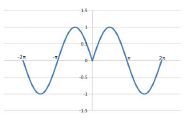
\includegraphics[width=0.35\textwidth]{figs/curveA.png}
        \item 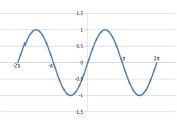
\includegraphics[width=0.35\textwidth]{figs/curveB.png}
        \item 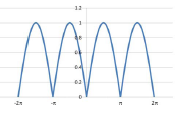
\includegraphics[width=0.35\textwidth]{figs/curveC.png}
        \item 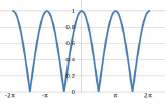
\includegraphics[width=0.35\textwidth]{figs/curveD.png}
    \end{enumerate}
    \caption{Different curve plots (A) to (D).}
    \label{fig:curves}
\end{figure}


\hfill{\brak{\text{GATE MN 2016}}}
\end{enumerate}

\vspace{2em}
\begin{center}
    \textbf{\textsc{END OF THE QUESTION PAPER}}
\end{center}
\newpage


\newpage
% Q1
\noindent \textbf{Q.1 -- Q.25 carry one mark each.}
\begin{enumerate}
\item The differential of the equation, $x^2 + y^2 = 1$, with respect to $x$ is
  \begin{enumerate}
    \begin{multicols}{4}
      \item $-x/y$
      \item $x/y$
      \item $-y/x$
      \item $y/x$
    \end{multicols}
  \end{enumerate}
  \hfill{\brak{\text{GATE MN 2016}}}
%Q2
\item If $[A][B] = [I]$ then
  \begin{enumerate}
\begin{multicols}{4}
      \item $[B] = [A]^T$
      \item $[A] = [B]^T$
      \item $[B] = [A]^{-1}$
      \item $[B] = [A]$
    \end{multicols}
  \end{enumerate}
  \hfill{\brak{\text{GATE MN 2016}}}
%Q3
\item $X^4 + C$ is the general integral of
  \begin{enumerate}
\begin{multicols}{4}
      \item $3\displaystyle\int x^3\,dx$
      \item $\displaystyle\frac{1}{4} \int x^3\,dx$
      \item $\displaystyle\int x^3\,dx$
      \item $4\displaystyle\int x^3\,dx$
    \end{multicols}
  \end{enumerate}
  \hfill{\brak{\text{GATE MN 2016}}}



% Q4
\item $\sinh(x)$ is
  \begin{enumerate}
\begin{multicols}{4}
      \item $\dfrac{e^x - e^{-x}}{4}$
      \item $\dfrac{e^x - e^{-x}}{2}$
      \item $\dfrac{e^x + e^{-x}}{2}$
      \item $\dfrac{e^x + e^{-x}}{4}$
    \end{multicols}
  \end{enumerate}
  \hfill{\brak{\text{GATE MN 2016}}}
  
%Q5
\item Identify the correct statement. \\
NONEL is used for surface connection of the blast holes in order to
  \begin{enumerate}
\item achieve better water resistance over detonating fuse
      \item have a precise delay timing
      \item provide noiseless shock front movement
      \item avoid deflagration
  \end{enumerate}

  \hfill{\brak{\text{GATE MN 2016}}}

% Q6
\item Identify the pattern of surface blasting given in the figure. 
The values of delay time, in ms, are given against each blasthole.

\begin{figure}[h!]
    \centering
    \includegraphics[width=0.9\linewidth]{figs/blast.png}
    \caption{blast.}
    \label{fig:blast}
\end{figure}

\begin{enumerate}
\begin{multicols}{2}
    \item V-cut
    \item extended V-cut
    \item row to row
    \item en echelon
  \end{multicols}
\end{enumerate}
\hfill{\brak{\text{GATE MN 2016}}}

% Q7
\item Identify the initiation sequence which is \textbf{NOT} possible for surface blasting.
  \begin{enumerate}
\item Detonating fuse $\Rightarrow$ Nonel $\Rightarrow$ Electronic detonator
      \item Electric detonator $\Rightarrow$ Nonel $\Rightarrow$ Detonating fuse
      \item Electric detonator $\Rightarrow$ Detonating fuse $\Rightarrow$ Nonel
      \item Electronic detonator $\Rightarrow$ Detonating fuse $\Rightarrow$ Nonel
  \end{enumerate}
  \hfill{\brak{\text{GATE MN 2016}}}

%Q8
\item Parallel holes at right angles to the face with some holes uncharged are associated with the following shot hole pattern
\vspace{-\baselineskip} 
  \begin{enumerate}
\begin{multicols}{4}
      \item drag cut
      \item wedge cut
      \item pyramid cut
      \item burn cut
    \end{multicols}
  \end{enumerate}
  \vspace{-\baselineskip} 
  \hfill{\brak{\text{GATE MN 2016}}}
%Q9
\item Bieniawski’s Rock Mass Rating considers the parameters: RQD, spacing of joints, condition of joints, ground water condition, and
\vspace{-\baselineskip} 
  \begin{enumerate}
\begin{multicols}{1}
      \item tensile strength
      \item uniaxial compressive strength
      \item shear strength
      \item buckling strength
    \end{multicols}
  \end{enumerate}
  \vspace{-\baselineskip} 
  \hfill{\brak{\text{GATE MN 2016}}}

% Q10
\item A rockmass is subjected to hydrostatic pressure of $6$ MPa. If each of the measured strains 
$\varepsilon_{xx} = \varepsilon_{yy} = \varepsilon_{zz}$ is $2.0$ mm/m, then the bulk modulus, in GPa, is \underline{\hspace{1.5cm}}.
\begin{flushright}
{\brak{\text{GATE MN 2016}}}
\end{flushright}

% Q11
\item Identify the uniaxial compressive loading condition from the following four Mohr circles.
\begin{figure}[h!]
    \centering
    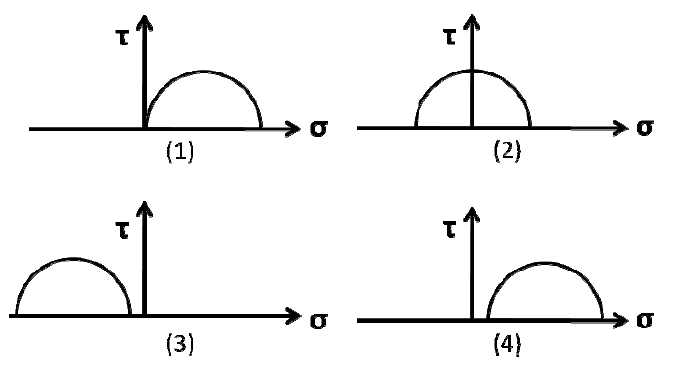
\includegraphics[width=0.7\linewidth]{figs/mohr_circles.png}
    \caption{mohr circles.}
    \label{fig:mohr_circles}
\end{figure}

%Q11
\begin{enumerate}
\begin{multicols}{4}
    \item (1)
    \item (2)
    \item (3)
    \item (4)
  \end{multicols}
\end{enumerate}
  \hfill{\brak{\text{GATE MN 2016}}}

% Q12
\item Out of the given stress–strain curves, identify the rock type that is most prone to rock burst.

\begin{figure}[h!]
    \centering
    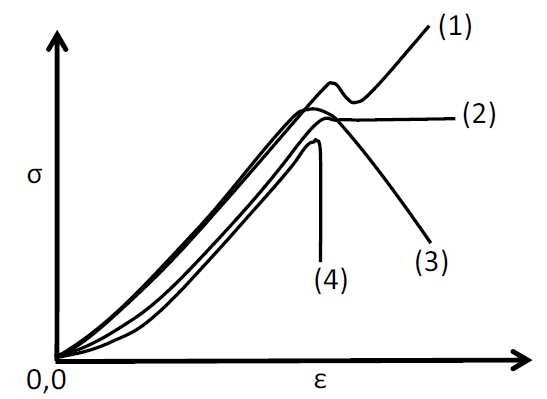
\includegraphics[width=0.7\linewidth]{figs/stress_strain.png}
    \caption{stress strain.}
    \label{fig:stress_strain}
\end{figure}

\begin{enumerate}
\begin{multicols}{4}
    \item (1)
    \item (2)
    \item (3)
    \item (4)
  \end{multicols}
\end{enumerate}
\hfill{\brak{\text{GATE MN 2016}}}

% Q13
\item A longwall panel of width $120$ m is extracted at a depth of $200$ m. Critical subsidence is reached when the panel length becomes $150$ m. If the seam were to be worked at a depth of $300$ m, critical subsidence would be observed at a panel length, in m, of \underline{\hspace{1.5cm}}.

  \hfill{\brak{\text{GATE MN 2016}}}

% Q14
\item The support system followed along the goaf edge in a depillaring panel is
  \begin{enumerate}
\item rope stitching
      \item cable bolting
      \item wooden/steel chock
      \item hydraulic prop
  \end{enumerate}
  \hfill{\brak{\text{GATE MN 2016}}}
% Q15
\item Which one of the following ropes \textbf{CANNOT} be an effective cable bolt?
  \begin{enumerate}
\item locked coil wire rope
      \item Langs lay wire rope
      \item ordinary lay wire rope
      \item bird-caged wire rope
  \end{enumerate}
  \hfill{\brak{\text{GATE MN 2016}}}
% Q16
\item In metalliferous mines, the sublevel interval does \textbf{NOT} depend on
  \begin{enumerate}
\item capacity of drilling equipment
      \item capacity of loading equipment
      \item strength of rib pillar
      \item strength of wall rock
  \end{enumerate}
  \hfill{\brak{\text{GATE MN 2016}}}

% Q17
\item Jack hammer does \textbf{NOT} contain
  \begin{enumerate}
\item pawl and ratchet
      \item gear box
      \item rifle bar
      \item piston
  \end{enumerate}
  \hfill{\brak{\text{GATE MN 2016}}}
% Q18
\item At the inlet of a mine roadway, the dry and wet bulb temperatures of air are $38^{\circ}\mathrm{C}$ and $29^{\circ}\mathrm{C}$, respectively. At the outlet, the corresponding temperatures are $32^{\circ}\mathrm{C}$ and $29^{\circ}\mathrm{C}$, respectively. The process of heat transfer in the airway is described as
  \begin{enumerate}
\item evaporative cooling
      \item sensible cooling
      \item sensible heating
      \item dehumidification
  \end{enumerate}
  \hfill{\brak{\text{GATE MN 2016}}}
% Q19
\item Underground coal mines are in principle ventilated by exhausting system, so that
  \begin{enumerate}
\item spontaneous heating risk is reduced
      \item fumes can be quickly removed in case of an underground fire
      \item build-up of methane concentration is decreased
      \item cool and fresh intake air can enter underground
  \end{enumerate}
  \hfill{\brak{\text{GATE MN 2016}}}

% Q20
\item Identify the WRONG statement. \\
Pit bottom air lock
  \begin{enumerate}
\item prevents the short circuiting of air when the flow is reversed in coal mines
      \item has at least three doors
      \item has at least one door that has provision for latching
      \item all doors are in principle designed to open towards high pressure side of the air
  \end{enumerate}
  \hfill{\brak{\text{GATE MN 2016}}}
% Q21
\item Identify the WRONG statement. \\
The ``temperature inversion'' of the atmosphere in surface mines aggravates the problem of
  \begin{enumerate}
\item airborne dust
      \item noise
      \item ground vibrations
      \item visibility
  \end{enumerate}

  \hfill{\brak{\text{GATE MN 2016}}}
% Q22
\item In a CO self rescuer, the purpose of the calcium bromide and lithium chloride mixture is to
  \begin{enumerate}
\item dry the incoming air
      \item convert the CO catalytically to CO$_2$
      \item absorb and thereby neutralise CO
      \item cool the inhaled air from excess exothermic heat due to chemical reaction
  \end{enumerate}
  \hfill{\brak{\text{GATE MN 2016}}}
% 23
\item IRR of a project is the discount rate at which
  \begin{enumerate}
\item profit after tax is zero
      \item written down value of the project is zero
      \item revenue from the project is zero
      \item NPV is zero
  \end{enumerate}
\hfill{\brak{\text{GATE MN 2016}}}
%24
\item For the critical path network shown, the slack for the activity `b', in months, is

\begin{figure}[h!]
    \centering
    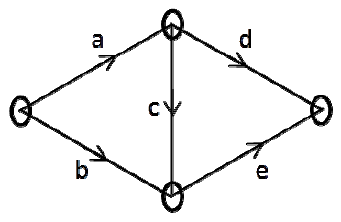
\includegraphics[width=\linewidth]{figs/network.png}
    \caption{network.}
    \label{fig:network}
\end{figure}

\begin{enumerate}
\begin{multicols}{4}
    \item 4
    \item 6
    \item 9
    \item 13
  \end{multicols}
\end{enumerate}
\hfill{\brak{\text{GATE MN 2016}}}

%25
\item The three axes comprising the numerical codification of resources, as per the UNFC, are
  \begin{enumerate}
\item Economic Viability, Geological Assessment, Geotechnical Assessment
      \item Geological Assessment, Environmental Assessment, Feasibility Assessment
      \item Feasibility Assessment, Geological Assessment, Mining Assessment
      \item Economic Viability, Geological Assessment, Feasibility Assessment
  \end{enumerate}
  \hfill{\brak{\text{GATE MN 2016}}}

\vspace{1em}
\noindent\textbf{Q.26 -- Q.55 carry two marks each.}

\item Equations of two planes are $z = 4$ and $z = 4 + 3x$. The included angle between the two planes in degrees, is \underline{\hspace{2cm}}.
\hfill{\brak{\text{GATE MN 2016}}}

\item A force $\vec{P} = 2\hat{i} - 5\hat{j} + 6\hat{k}$ acts on a particle. The particle is moved from point A to point B, where the position vectors of $\vec{A}$ and $\vec{B}$ are $6\hat{i} + \hat{j} - 3\hat{k}$ and $4\hat{i} - 3\hat{j} - 2\hat{k}$ respectively. The work done is \underline{\hspace{2cm}}.

\hfill{\brak{\text{GATE MN 2016}}}

%28
\item The value of $x$ in the simultaneous equations is \underline{\hspace{2cm}}
\[
\begin{aligned}
3x + y + 2z &= 3 \\
2x - 3y - z &= -3 \\
x + 2y + z &= 4
\end{aligned}
\]

\hfill{\brak{\text{GATE MN 2016}}}

%29
\item Two persons $P$ and $Q$ toss an unbiased coin alternately on an understanding that whoever gets the head first wins. If $P$ starts the game, then the probability of $P$ winning the game is \underline{\hspace{2cm}}.
\hfill{\brak{\text{GATE MN 2016}}}
%30
\item Data pertaining to a surface bench blast is given below:  
\begin{tabular}{ll}
Burden = 3.0 m & Sub-grade drilling = 1.0 m \\
Spacing = 4.0 m & Collar stemming = 4.0 m \\
Bench height = 10.0 m & Air decking length = 1.0 m \\
Density of rock = $2000 \ \text{kg/m}^3$ & Linear charge concentration = $10 \ \text{kg/m}$ \\
\end{tabular}


\vspace{0.5em}
The powder factor of the blast, in kg/tonne, is \underline{\hspace{2cm}}.
\hfill{\brak{\text{GATE MN 2016}}}
%31
\item Match the following for a typical slurry explosive.  

\begin{center}
\begin{tabular}[12pt]{ |c|l|c|l| } 
    \hline
    \textbf{Chemical} &  & \textbf{Purpose} &  \\ 
    \hline
    P. & Calcium nitrate & 1. & Cross linking agent \\ 
    \hline 
    Q. & Potassium dichromate & 2. & Gelling agent \\ 
    \hline
    R. & TNT & 3. & Oxidiser \\ 
    \hline   
    S. & Starch & 4. & Fuel \\ 
    \hline
\end{tabular}


\end{center}

\begin{enumerate}
\item P-1, Q-2, R-3, S-4
    \item P-2, Q-4, R-3, S-1
    \item P-3, Q-1, R-4, S-2
    \item P-4, Q-3, R-2, S-1
\end{enumerate}
\hfill{\brak{\text{GATE MN 2016}}}

%32
\item A $10$ m thick coal block is excavated by a contractor at a cost of Rs.\ $40$ per m$^3$. 
The excavated area, measured in the mine plan, is found to be $50\ \mathrm{cm}^2$. 
If the mine plan has been drawn to a scale of $1\!:\!1000$, the payment to be made to the contractor, 
in lakhs of Rs., is \underline{\hspace{2cm}}.
\hfill{\brak{\text{GATE MN 2016}}}

%33
\item Two vertical shafts of a mine have the following parameters:

\begin{center}
\renewcommand{\arraystretch}{1.2}
\begin{tabular}[12pt]{ |c|c|c| }
    \hline
    \textbf{Shaft} & \textbf{Shaft-A} & \textbf{Shaft-B} \\
    \hline
    Collar RL (m) & 0.0 & 0.0 \\
    \hline
    Depth (m) & 250 & 200 \\
    \hline
    Northing (m) & 200 & 100 \\
    \hline
    Easting (m) & 100 & $-100$ \\
    \hline
\end{tabular}

\end{center}

The gradient of the drift connecting the shaft bottoms, in degrees, is \underline{\hspace{2cm}}.
\hfill{\brak{\text{GATE MN 2016}}}

%34
\item For a station `A' on the Earth's surface, as shown in the figure, match the following

\begin{figure}[h!]
    \centering
    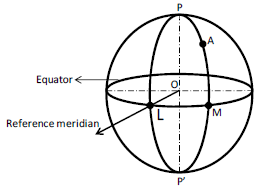
\includegraphics[width=0.35\linewidth]{figs/earth.png}
    \caption{earth.}
    \label{fig:earth}
\end{figure}

\begin{center}
\begin{minipage}{0.45\linewidth}
\centering
\renewcommand{\arraystretch}{1.2}
\begin{tabular}[12pt]{ |c|l| }
  \hline
  \textbf{Arc} & \\ \hline
  Q. & MA \\ \hline
  R. & LM \\ \hline
  S. & PA \\ \hline
\end{tabular}

\end{minipage}\hfill
\begin{minipage}{0.45\linewidth}
\centering
\renewcommand{\arraystretch}{1.2}
\begin{tabular}[12pt]{ |c|l| }
  \hline
  \textbf{Description} & \\ \hline
  1. & Longitude \\ \hline
  2. & Co-latitude \\ \hline
  3. & Latitude \\ \hline
\end{tabular}

\end{minipage}
\end{center}

\begin{enumerate}
\begin{multicols}{4}
    \item Q-2, R-3, S-1
    \item Q-3, R-1, S-2
    \item Q-2, R-1, S-3
    \item Q-3, R-2, S-1
  \end{multicols}
\end{enumerate}
\hfill{\brak{\text{GATE MN 2016}}}

%35
\item Match the following for the prismatic compass shown below

\begin{figure}[h!]
    \centering
    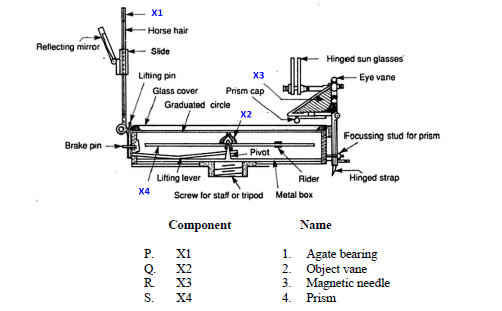
\includegraphics[width=0.75\linewidth]{figs/prismatic_compass.png}
    \caption{prismatic compass.}
    \label{fig:prismatic_compass}
\end{figure}

\begin{center}
\begin{minipage}{0.45\linewidth}
\centering
\renewcommand{\arraystretch}{1.2}
\begin{tabular}[12pt]{ |c|l| }
  \hline
  \textbf{Component} & \\ \hline
  P. & X1 \\ \hline
  Q. & X2 \\ \hline
  R. & X3 \\ \hline
  S. & X4 \\ \hline
\end{tabular}

\end{minipage}\hfill
\begin{minipage}{0.45\linewidth}
\centering
\renewcommand{\arraystretch}{1.2}
\begin{tabular}[12pt]{ |c|l| }
  \hline
  \textbf{Name} & \\ \hline
  1. & Agate bearing \\ \hline
  2. & Object vane \\ \hline
  3. & Magnetic needle \\ \hline
  4. & Prism \\ \hline
\end{tabular}

\end{minipage}
\end{center}

\begin{enumerate}
\item P-1, Q-2, R-3, S-4
    \item P-1, Q-3, R-2, S-4
    \item P-2, Q-1, R-4, S-3
    \item P-3, Q-1, R-4, S-2
\end{enumerate}
\hfill{\brak{\text{GATE MN 2016}}}

%36
\item A ladder placed against a frictionless wall at an inclination of $60^\circ$ with horizontal, is in a state of limiting equilibrium. The ladder has a length of $13$ m and a uniform mass of $4\ \mathrm{kg/m}$. The coefficient of friction between the ladder and the floor is \underline{\hspace{2cm}}.
\hfill{\brak{\text{GATE MN 2016}}}

%37
\item A cubical rock sample is enclosed between two fixed hard steel plates as shown in the figure below.
The modulus of elasticity and Poisson’s ratio of the rock are $2\ \text{GPa}$ and $0.25$, respectively.
If the rock is subjected to the stresses as shown in the figure, the strain in $x$-direction, in mm/m, is \underline{\hspace{2cm}}.

\begin{figure}[h!]
    \centering
    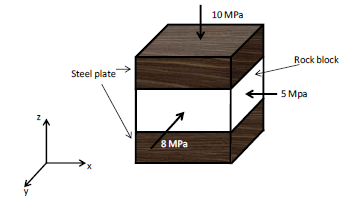
\includegraphics[width=0.55\linewidth]{figs/rock_cube.png}
    \caption{rock cube.}
    \label{fig:rock_cube}
\end{figure}
\hfill{\brak{\text{GATE MN 2016}}}
%38
\item In a hydrostatic stress field, point $A$ is in the middle of two circular openings as shown in the figure.
The radial stress, in MPa, at point $A$ is \underline{\hspace{2cm}}.

\begin{figure}[h!]
    \centering
    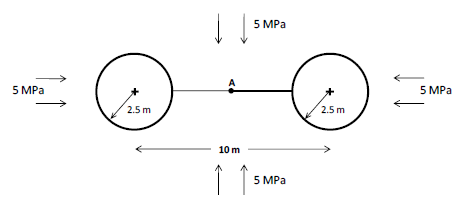
\includegraphics[width=0.65\linewidth]{figs/openings.png}
    \caption{openings.}
    \label{fig:openings}
\end{figure}
\hfill{\brak{\text{GATE MN 2016}}}
%39
\item Curves (a) and (b) represent the stress distributions along the length of a `full column grouted bolt' shown in the figure. Curves (a) and (b) are

\begin{figure}[h!]
    \centering
    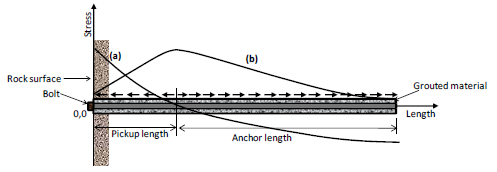
\includegraphics[width=0.75\linewidth]{figs/grounded_bolt.png}
    \caption{grounded bolt.}
    \label{fig:grounded_bolt}
\end{figure}

\begin{enumerate}
\begin{multicols}{2}
    \item Tensile stress, Compressive stress
    \item Axial stress, Shear stress
    \item Compressive stress, Tensile stress
    \item Shear stress, Axial stress
  \end{multicols}
\end{enumerate}
\hfill{\brak{\text{GATE MN 2016}}}

%40
\item Match the following mechanical properties with the formulae

\begin{center}
\begin{minipage}{0.45\linewidth}
\centering
\renewcommand{\arraystretch}{1.2}
\begin{tabular}[12pt]{ |c|l| }
\hline
\textbf{Mechanical property} & \\ \hline
P. & Modulus of elasticity \\ \hline
Q. & Compressive strength \\ \hline
R. & Shear Strength \\ \hline
S. & Poisson’s ratio \\ \hline
\end{tabular}

\end{minipage}\hfill
\begin{minipage}{0.45\linewidth}
\centering
\renewcommand{\arraystretch}{1.2}
\begin{tabular}[12pt]{ |c|l| }
\hline
\textbf{Formula} & \\ \hline
1. & $c+\sigma_t \tan \varphi$ \\ \hline
2. & $\varepsilon_{\text{lateral}}/\varepsilon_{\text{longitudinal}}$ \\ \hline
3. & $\sigma/\varepsilon$ \\ \hline
4. & $F_s/(\pi r^2)$ \\ \hline
\end{tabular}

\end{minipage}
\end{center}

\begin{enumerate}
\item P-1, Q-2, R-3, S-4
    \item P-1, Q-3, R-2, S-4
    \item P-3, Q-4, R-1, S-2
    \item P-3, Q-2, R-1, S-4
\end{enumerate}
\hfill{\brak{\text{GATE MN 2016}}}

%41
\item A skip of $10$ tonne capacity hoists ore through a $1000$ m deep shaft at a speed of $20\ \text{m/s}$. 
The skip accelerates and decelerates at $2.0\ \text{m/s}^2$. The loading and unloading times for the skip are 
$2.5$ min and $1.5$ min, respectively. The maximum hourly capacity of the hoisting system, in tonnes, is 
\underline{\hspace{2.5cm}}.
\hfill{\brak{\text{GATE MN 2016}}}
\newpage
%42
\item Match the following:

\begin{center}
\begin{minipage}{0.45\linewidth}
\centering
\renewcommand{\arraystretch}{1.2}
\begin{tabular}[12pt]{ |c|l| }
\hline
\textbf{Haulage unit} & \\ \hline
P. & Friction winder \\ \hline
Q. & Drum winder \\ \hline
R. & Direct rope haulage \\ \hline
S. & Endless rope haulage \\ \hline
\end{tabular}

\end{minipage}\hfill
\begin{minipage}{0.45\linewidth}
\centering
\renewcommand{\arraystretch}{1.2}
\begin{tabular}[12pt]{ |c|l| }
\hline
\textbf{Safety device} & \\ \hline
1. & Run-away switch \\ \hline
2. & Lilly controller \\ \hline
3. & Regenerative braking \\ \hline
4. & Monkey/back catch \\ \hline
\end{tabular}

\end{minipage}
\end{center}

\begin{enumerate}
\item P-1, Q-2, R-3, S-4
    \item P-3, Q-2, R-1, S-4
    \item P-1, Q-3, R-4, S-2
    \item P-2, Q-3, R-1, S-4
\end{enumerate}
\hfill{\brak{\text{GATE MN 2016}}}

%43
\item In the gear assembly shown, the rpm of Gear 1 is $600$. 
The number of teeth in Gear 1, Gear 2, Gear 3, Gear 4, Gear 5 and Gear 6 is 
$30, 45, 15, 20, 10$ and $30$, respectively. 
The rpm of Gear 6 is \underline{\hspace{2cm}}.

\begin{figure}[h!]
    \centering
    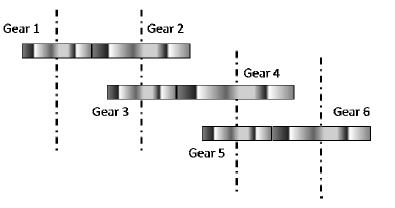
\includegraphics[width=0.75\linewidth]{figs/gears.png}
    \caption{gears.}
    \label{fig:gears}
\end{figure}
\hfill{\brak{\text{GATE MN 2016}}}

%44
\item An operating surface mine is proposed to be deepened by $30$ m as shown in the figure. 
If the density of the ore is $2.4\,\mathrm{tonne/m^3}$, the incremental stripping ratio for the deepening, 
in $\mathrm{m^3/tonne}$, is \underline{\hspace{2cm}}.

\begin{figure}[h!]
    \centering
    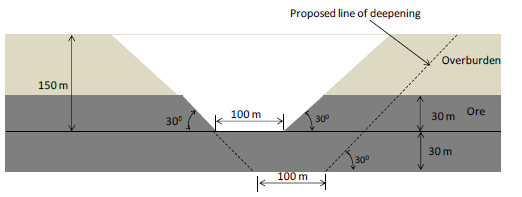
\includegraphics[width=0.85\linewidth]{figs/deepening.png}
    \caption{deepening.}
    \label{fig:deepening}
\end{figure}
\hfill{\brak{\text{GATE MN 2016}}}

%45
\item From an openpit sump, mine water is lifted using a $250$ m long straight pipeline laid along a
gradient of $34^\circ$. The pumping rate is $500$ gpm (1 gallon $= 3.8$ litres). Additional head loss due to
pipe friction can be considered to be $10\%$ of the head lifted. At an overall efficiency of $70\%$, the
electric power consumed by the pump, in kW, is \underline{\hspace{2cm}}.
\hfill{\brak{\text{GATE MN 2016}}}


%46
\item With reference to Coward diagram, match the following in the context of explosibility of a mixture of `normal air' and `methane'.

\begin{center}
\begin{minipage}{0.45\linewidth}
\centering
\renewcommand{\arraystretch}{1.2}
\begin{tabular}[12pt]{ |c|l| }
  \hline
  \textbf{(O$_2$ \%, CH$_4$ \%)} & \\ \hline
  P. & 20.5,\; 2.4 \\ \hline
  Q. & 19.0,\; 9.5 \\ \hline
  R. & 17.0,\; 19.0 \\ \hline
  S. & 20.0,\; 19.5 \\ \hline
\end{tabular}

\end{minipage}\hfill
\begin{minipage}{0.45\linewidth}
\centering
\renewcommand{\arraystretch}{1.2}
\begin{tabular}[12pt]{ |c|l| }
  \hline
  \textbf{Mixture status} & \\ \hline
  1. & Impossible mixture \\ \hline
  2. & Non-explosive \\ \hline
  3. & Potentially explosive \\ \hline
  4. & Explosive \\ \hline
\end{tabular}

\end{minipage}
\end{center}

\begin{enumerate}
\item P-2, Q-4, R-3, S-1
    \item P-2, Q-3, R-1, S-4
    \item P-2, Q-4, R-1, S-3
    \item P-3, Q-2, R-1, S-4
\end{enumerate}
\hfill{\brak{\text{GATE MN 2016}}}

%47
\item A U-tube manometer is subjected to differential pressure as shown. If specific gravity of kerosene is $0.8$, the value of $(P_1 - P_2)$, in Pa, is \underline{\hspace{1.5cm}}.

\begin{figure}[h!]
    \centering
    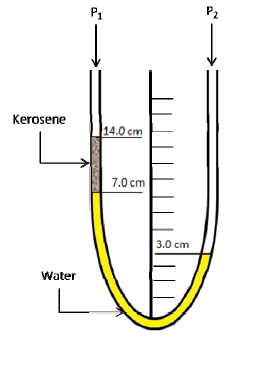
\includegraphics[width=0.65\linewidth]{figs/frame.png}
    \caption{frame.}
    \label{fig:frame}
\end{figure}

\hfill{\brak{\text{GATE MN 2016}}}
\newpage
%48
\item An air stream having an enthalpy of $100\ \mathrm{kJ/kg_{da}}$ is flowing at $20\ \mathrm{kg_{da}\,s^{-1}}$. 
It is cooled by water at temperature $10^{\circ}\mathrm{C}$ circulating in a cooling coil at a flow rate of 
$10.0\ \mathrm{L\,s^{-1}}$. If the return temperature of water is $20^{\circ}\mathrm{C}$, 
the enthalpy of the cooled air, in $\mathrm{kJ/kg_{da}}$, is \underline{\hspace{2cm}}.\\
{\footnotesize (Specific heat of water: $4.18\ \mathrm{kJ/(kg\,^{\circ}C)}$; kgda: kg of dry air.)}
\hfill{\brak{\text{GATE MN 2016}}}
 %49
\item The static pressure characteristic of a mine fan is as shown. If the mine resistance is $0.3\ \mathrm{Ns^2/m^8}$, 
the quantity generated by the fan, in $\mathrm{m^3/s}$, is \underline{\hspace{2cm}}.\\[0.2cm]
\begin{figure}[h!]
    \centering
    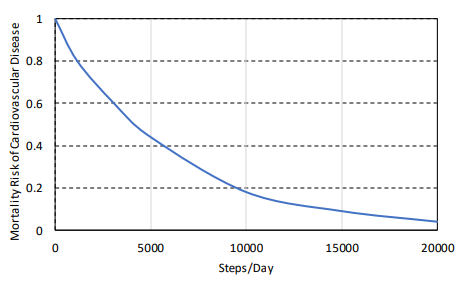
\includegraphics[width=0.65\linewidth]{figs/graph.png}
    \caption{graph.}
    \label{fig:graph}
\end{figure}
\hfill{\brak{\text{GATE MN 2016}}}

%50
\item In the context of ventilation plan symbols, match the following:

\begin{center}
\begin{minipage}{0.45\linewidth}
\centering
\renewcommand{\arraystretch}{1.4}
\begin{tabular}[12pt]{ |c|l| }
  \hline
  \textbf{Symbol} & \\ \hline
  P. & 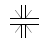
\includegraphics[height=1.5em]{figs/vplan1.png} \\ \hline   % <-- replace with your symbol image
  Q. & 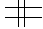
\includegraphics[height=1.5em]{figs/vplan2.png} \\ \hline   % <-- replace with your symbol image
  R. & 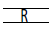
\includegraphics[height=1.5em]{figs/vplan3.png} \\ \hline   % <-- replace with your symbol image
  S. & 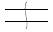
\includegraphics[height=1.5em]{figs/vplan4.png} \\ \hline   % <-- replace with your symbol image
\end{tabular}

\end{minipage}\hfill
\begin{minipage}{0.45\linewidth}
\centering
\renewcommand{\arraystretch}{1.2}
\begin{tabular}[12pt]{ |c|l| }
  \hline
  \textbf{Description} & \\ \hline
  1. & Temporary stopping \\ \hline
  2. & Regulator \\ \hline
  3. & Air-crossing \\ \hline
  4. & Ventilation stopping \\ \hline
\end{tabular}

\end{minipage}
\end{center}

\begin{enumerate}
\item P-3, Q-4, R-2, S-1
    \item P-2, Q-3, R-1, S-4
    \item P-1, Q-3, R-4, S-2
    \item P-3, Q-2, R-1, S-4
\end{enumerate}
\hfill{\brak{\text{GATE MN 2016}}}
\newpage
%51
\item A mill concentrate, having $25\%$ copper, is proposed to be sold at Rs.\ $1{,}25{,}000$ per tonne. 
The grade of the deposit is $0.8\%$ Cu and the overall cost of mining and milling is Rs.\ $2{,}520$ per tonne of ore. 
At a recovery of $75\%$, the estimated profit, in Rs./tonne of concentrate, is \underline{\hspace{2.2cm}}.
\hfill{\brak{\text{GATE MN 2016}}}

%52
\item Copper grade distribution in an ore body has the probability density function, $f(x)$, as shown in the figure.
The average grade of the deposit, in \% Cu, is \underline{\hspace{2cm}}.

\begin{figure}[h!]
    \centering
    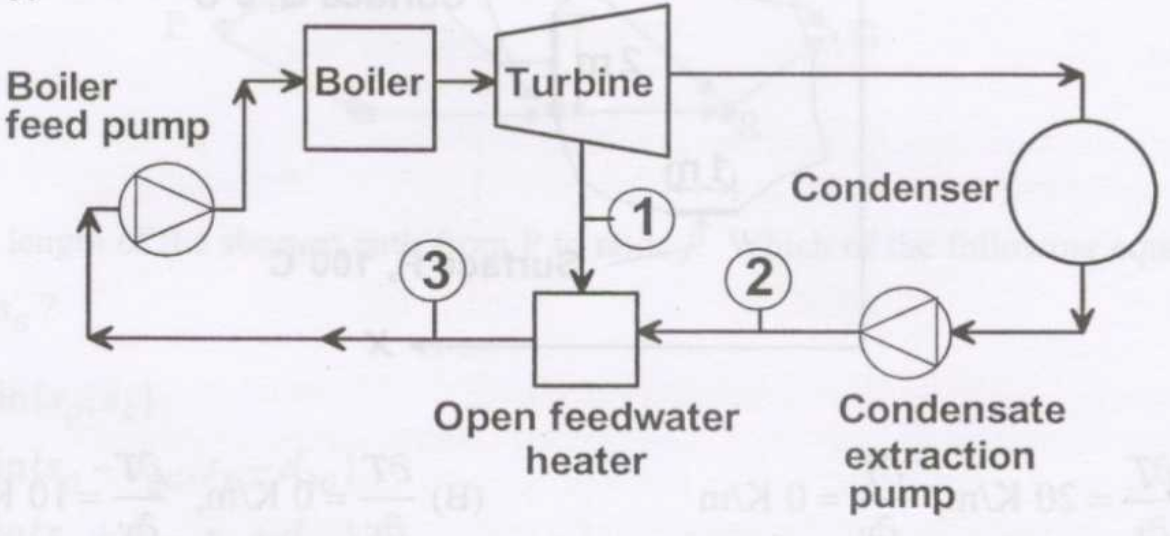
\includegraphics[width=0.55\linewidth]{figs/q52.png}
    \caption{q52.}
    \label{fig:q52}
\end{figure}
\hfill{\brak{\text{GATE MN 2016}}}
%53
\item The semivariogram shown belongs to a bauxite deposit. The expected difference in the Al$_2$O$_3$ (\%) values
between two boreholes separated by a distance of $200$ m is \underline{\hspace{2cm}}.

\begin{figure}[h!]
    \centering
    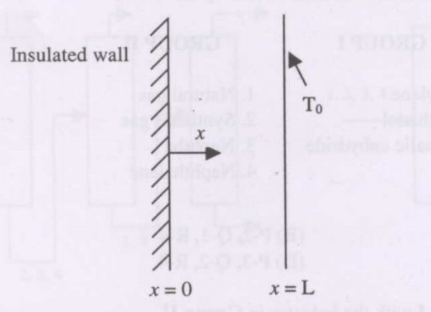
\includegraphics[width=0.55\linewidth]{figs/q53.png}
    \caption{q53.}
    \label{fig:q53}
\end{figure}
\hfill{\brak{\text{GATE MN 2016}}}

%54
\item A surface mine has $15$ identical dumpers and two shovels. For shovel 1, the dumper cycle time is 
$30$ min and the shovel loading time is $5$ min. For shovel 2, the dumper cycle time is $32$ min and the 
shovel loading time is $4.0$ min. Based on match factor optimisation (equitable match factor), the ideal 
allocation of dumpers to shovel 1 and shovel 2, respectively, is
  \begin{enumerate}
\begin{multicols}{4}
      \item 6, 9
      \item 7, 8
      \item 9, 6
      \item 8, 7
    \end{multicols}
  \end{enumerate}
\hfill{\brak{\text{GATE MN 2016}}}
%55
\item The composited grade value, in \%, between the RLs $10$ m to $20$ m for the following borehole configuration is \underline{\hspace{2cm}}.

\begin{figure}[h!]
    \centering
    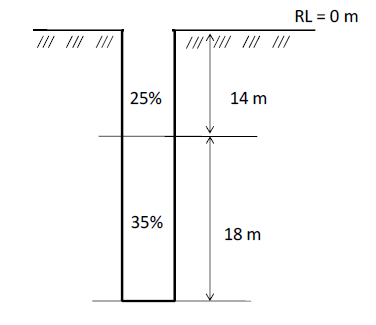
\includegraphics[width=0.6\linewidth]{figs/borehole.png}
    \caption{borehole.}
    \label{fig:borehole}
\end{figure}
\hfill{\brak{\text{GATE MN 2016}}}
\vspace{2em}
\begin{center}
    \textbf{\textsc{END OF THE QUESTION PAPER}}
\end{center}
\end{enumerate}
\end{document}